\chapter{Implementation\label{cha:chapter5}}

This chapter describes the implementation of component X. Three systems were chosen as reference implementations: a desktop version for Windows and Linux PCs, a Windows Mobile version for Pocket PCs and a mobile version based on Android. 

\section{Completing the Scale Tezos Blockchain with Zk-Rollups project}
This section explains the implementation of the remaining features of the \textit{Scale Tezos Blockchain using Zk-Rollups} project. Since some other already-implemented features have been modified, this section also explains the changes made to those features to integrate the new changes made

\subsection{Storage}

Originally the storage has been designed to hold a limited amount of users, thus using a normal Map. It was composed by:
\begin{itemize}
	\item A Map of accounts indexed by a natural number containing:
		\begin{itemize}
			\item A public key;
			\item A balance.
		\end{itemize}
	\item A list of 8 scalar values representing the Merkle Tree root of the accounts public keys;
	\item A list of 8 scalar values representing the Merkle Tree root of the accounts balances.
\end{itemize}

Having as objective the system to be scalable the storage has been modified to support a growing number of users using a Big Map. This is a key difference because the Big Map is lazily deserialized\footnote{\url{https://tezos.gitlab.io/michelson-reference/\#type-big_map}}, not having to use gas during a contract call to deserialize all the accounts Map. The storage is now composed by:
\begin{itemize}
	\item A Big Map of accounts indexed by a natural number containing:
		\begin{itemize}
			\item A public key;
			\item A balance;
			\item A nonce.
		\end{itemize}
	\item A list of 8 scalar values representing the Merkle Tree root of the accounts public keys;
	\item A list of 8 scalar values representing the Merkle Tree root of the accounts balances concatenated to their respective nonces.
\end{itemize}

The nonce mechanism and the Merkle Tree roots are explained in the section \ref{subsec:merkletreeBalanceNonce}.

\subsection{Balance and Nonce Merkle Tree}
\label{subsec:merkletreeBalanceNonce}

To avoid the possible attack of having an user sending repeatedly the same transaction the nonce mechanism is used: the nonce is a propriety stored in the account Big Map, saved on Layer 1. Every time an user wants to submit a transaction the new transaction must include a nonce incremented by one. This allows to check if the transaction has been already executed.

To prove inside the Zokrates environment that we're using the updated version of balances and nonces a merkle tree of the lists must be computed. This merkle tree should be computed for both the balances and nonces lists passed as parameters. This adds complexity because we have to compute two full binary trees. The workaround to this problem is to concatenate and hash the balances and nonces for each user and compute a single merkle tree of them. The concatenation of balances and nonces is done by hashing the concatenation of the balances and nonces themselves with sha256. This returns a 32 bytes hash that is used as the input of the merkle tree leaf for an user. This approach adds only the complexity of the concatenation function that performs a number of hashes equal to the number of accounts, but still having proven that the balances and nonces are updated.

\subsection{Rollup execution}

The rollup execution has been changed to include the calculation of the new nonces of the users when calculating the new balances.
A precondition that must be respected is that Zokrates receives the transaction ordered by nonce for a user. It can receive transactions from different users but the transactions of a single user must be ordered by nonce. The algorithm that checks the transaction nonces and calculates the new nonces is the following:
\begin{itemize}
	\item Create a new array X copying the old nonce array;
	\item Iterate over the transactions:
	\item \begin{itemize}
		\item Check in X if the transaction nonce for the sender is equal to the nonce of the user added one;
		\item If it is, increment the nonce of the user in the array X and continue;
		\item If it is not, fail execution.
    \end{itemize}
\end{itemize}

This allows to receive multiple transactions from the same user while avoiding a duplicate transaction to be applied.

No relevant overhead is added to the complexity of the rollup execution because the nonce check is done in the same loop of the balance calculation and accessing directly to the array, it is still O(n).



\subsection{Registration and Deregistration}

This section describes the registration and deregistration process of a user. The main idea is to insert and remove users from the storage, leaving empty fake users in case of a deregistration. This is made in order to preserve the position of the users inside the storage.
\label{subsec:registration}

To register a new user, two Merkle Trees must be recalculated with the new user's public key, balance and nonce. This computation is done inside a Zokrates program that returns the new root hashes of the Merkle Trees. The new root hashes are then passed to the contract that updates the storage with the new root hashes. The Zokrates program expects the exact position where to put the new data of the new user. This position is calculated from the external manager that can contact an rpc and compute the first empty slot inside the Big Map of the storage. The register process checks if at the specified position the account has an empty key, balance and nonce set to 0. After the initial checks it sets the nonce at the value of 1, the balance at the value of 0 and the public key at the value of the public key of the user.

\subsection{Deregistration}

The deregistration process is similar to the registration process described at \ref{subsec:registration}. The 


\section{Project Structure\label{sec:projectstructure}}

The implementation is separated into 2 distinguished eclipse projects as depicted in figure \ref{fig:projects}.

\begin{figure}[htb]
  \centering
  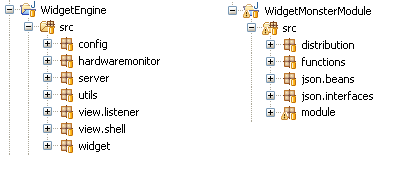
\includegraphics[width=10cm]{screenshot_2_projects}
  \caption{Project Structure}
  \label{fig:projects}
\end{figure}

\noindent
The following listing briefly describes the single packages of both projects in alphabetical order to give an overview of the implementation:
\\
\\
\textbf{config} 
\\
Lorem Ipsum...
\\
\\
\textbf{server} 
\\
Lorem Ipsum...
\\
\\
\textbf{utils} 
\\
Lorem Ipsum...

\section{Important Implementation Aspects\label{sec:implaspects}}

Do not explain every class in detail. Give a short introduction about the modules or the eclipse projects. If you want to explain relevant code snippets use the 'lstlisting' tag of LaTeX. Put only short snippets into your thesis. Long listing should be part of the annex.

\lstset{caption=JSON String Code Snippet,label=jsonstring,showstringspaces=false}
\begin{lstlisting}
{
	id: 1,
	method: "myInstance.getGroup",
	params: ["Teammates", 2, true]
}

{
	id: 2,
	result: [
		  "groupDesc":"These are my teammates",
		  {
			"javaClass":"src.package.MemberClass",
			"memberName": "Bob",      
		  }
		]
}\end{lstlisting}

You can also compare different approaches. Example: Since the implementation based on X failed I choosed to implement the same aspect based on Y. The new approach resulted in a much faster ...

\section{Graphical User Interface\label{sec:gui}}

Lorem Ipsum...

\section{Documentation\label{sec:docu}}

Lorem Ipsum...


